\documentclass[11pt, a4paper]{article}
\usepackage[utf8]{inputenc}
\usepackage{graphicx}
\usepackage{fancyhdr}
\usepackage{tikz}
\usepackage{float}
\graphicspath{{./images/}}

\usepackage{gfsartemisia-euler}
\usepackage[T1]{fontenc}

\usepackage{listings}

%%%%%%%%%%%%%%%%%%%%%%%%%%%%%%%%%%%%%%%%%%%%%%
%%%%%%%%%%          CONFIG          %%%%%%%%%%
\newcommand{\settingsTitle}{Title}
\newcommand{\settingsFirstName}{First}
\newcommand{\settingsLastName}{Last}
\newcommand{\settingsMonth}{Month}
\newcommand{\settingsYear}{Year}
\newcommand{\settingsCourseDept}{Dept}
\newcommand{\settingsCourseNum}{Num} % DON'T FORGET `\_'
\newcommand{\settingsQuarter}{Quarter}
%%%%%%%%%%          CONFIG          %%%%%%%%%%
%%%%%%%%%%%%%%%%%%%%%%%%%%%%%%%%%%%%%%%%%%%%%%

% create title
\title{\settingsTitle}
\author{\settingsFirstName\,\settingsLastName}
\date{\settingsMonth\,\settingsYear}

\begin{document}

% set pagestyle
\pagestyle{fancy}
\setlength{\headheight}{14pt}

% clear header
\fancyhead{}

% set header
\fancyhead[L]{\settingsCourseDept\,\settingsCourseNum\, | \settingsQuarter\,\settingsYear}
\fancyhead[R]{\settingsLastName}

% homework title
\maketitle
% ensure titlepage has same style
\thispagestyle{fancy}

\begin{figure}[H]
    \centering
    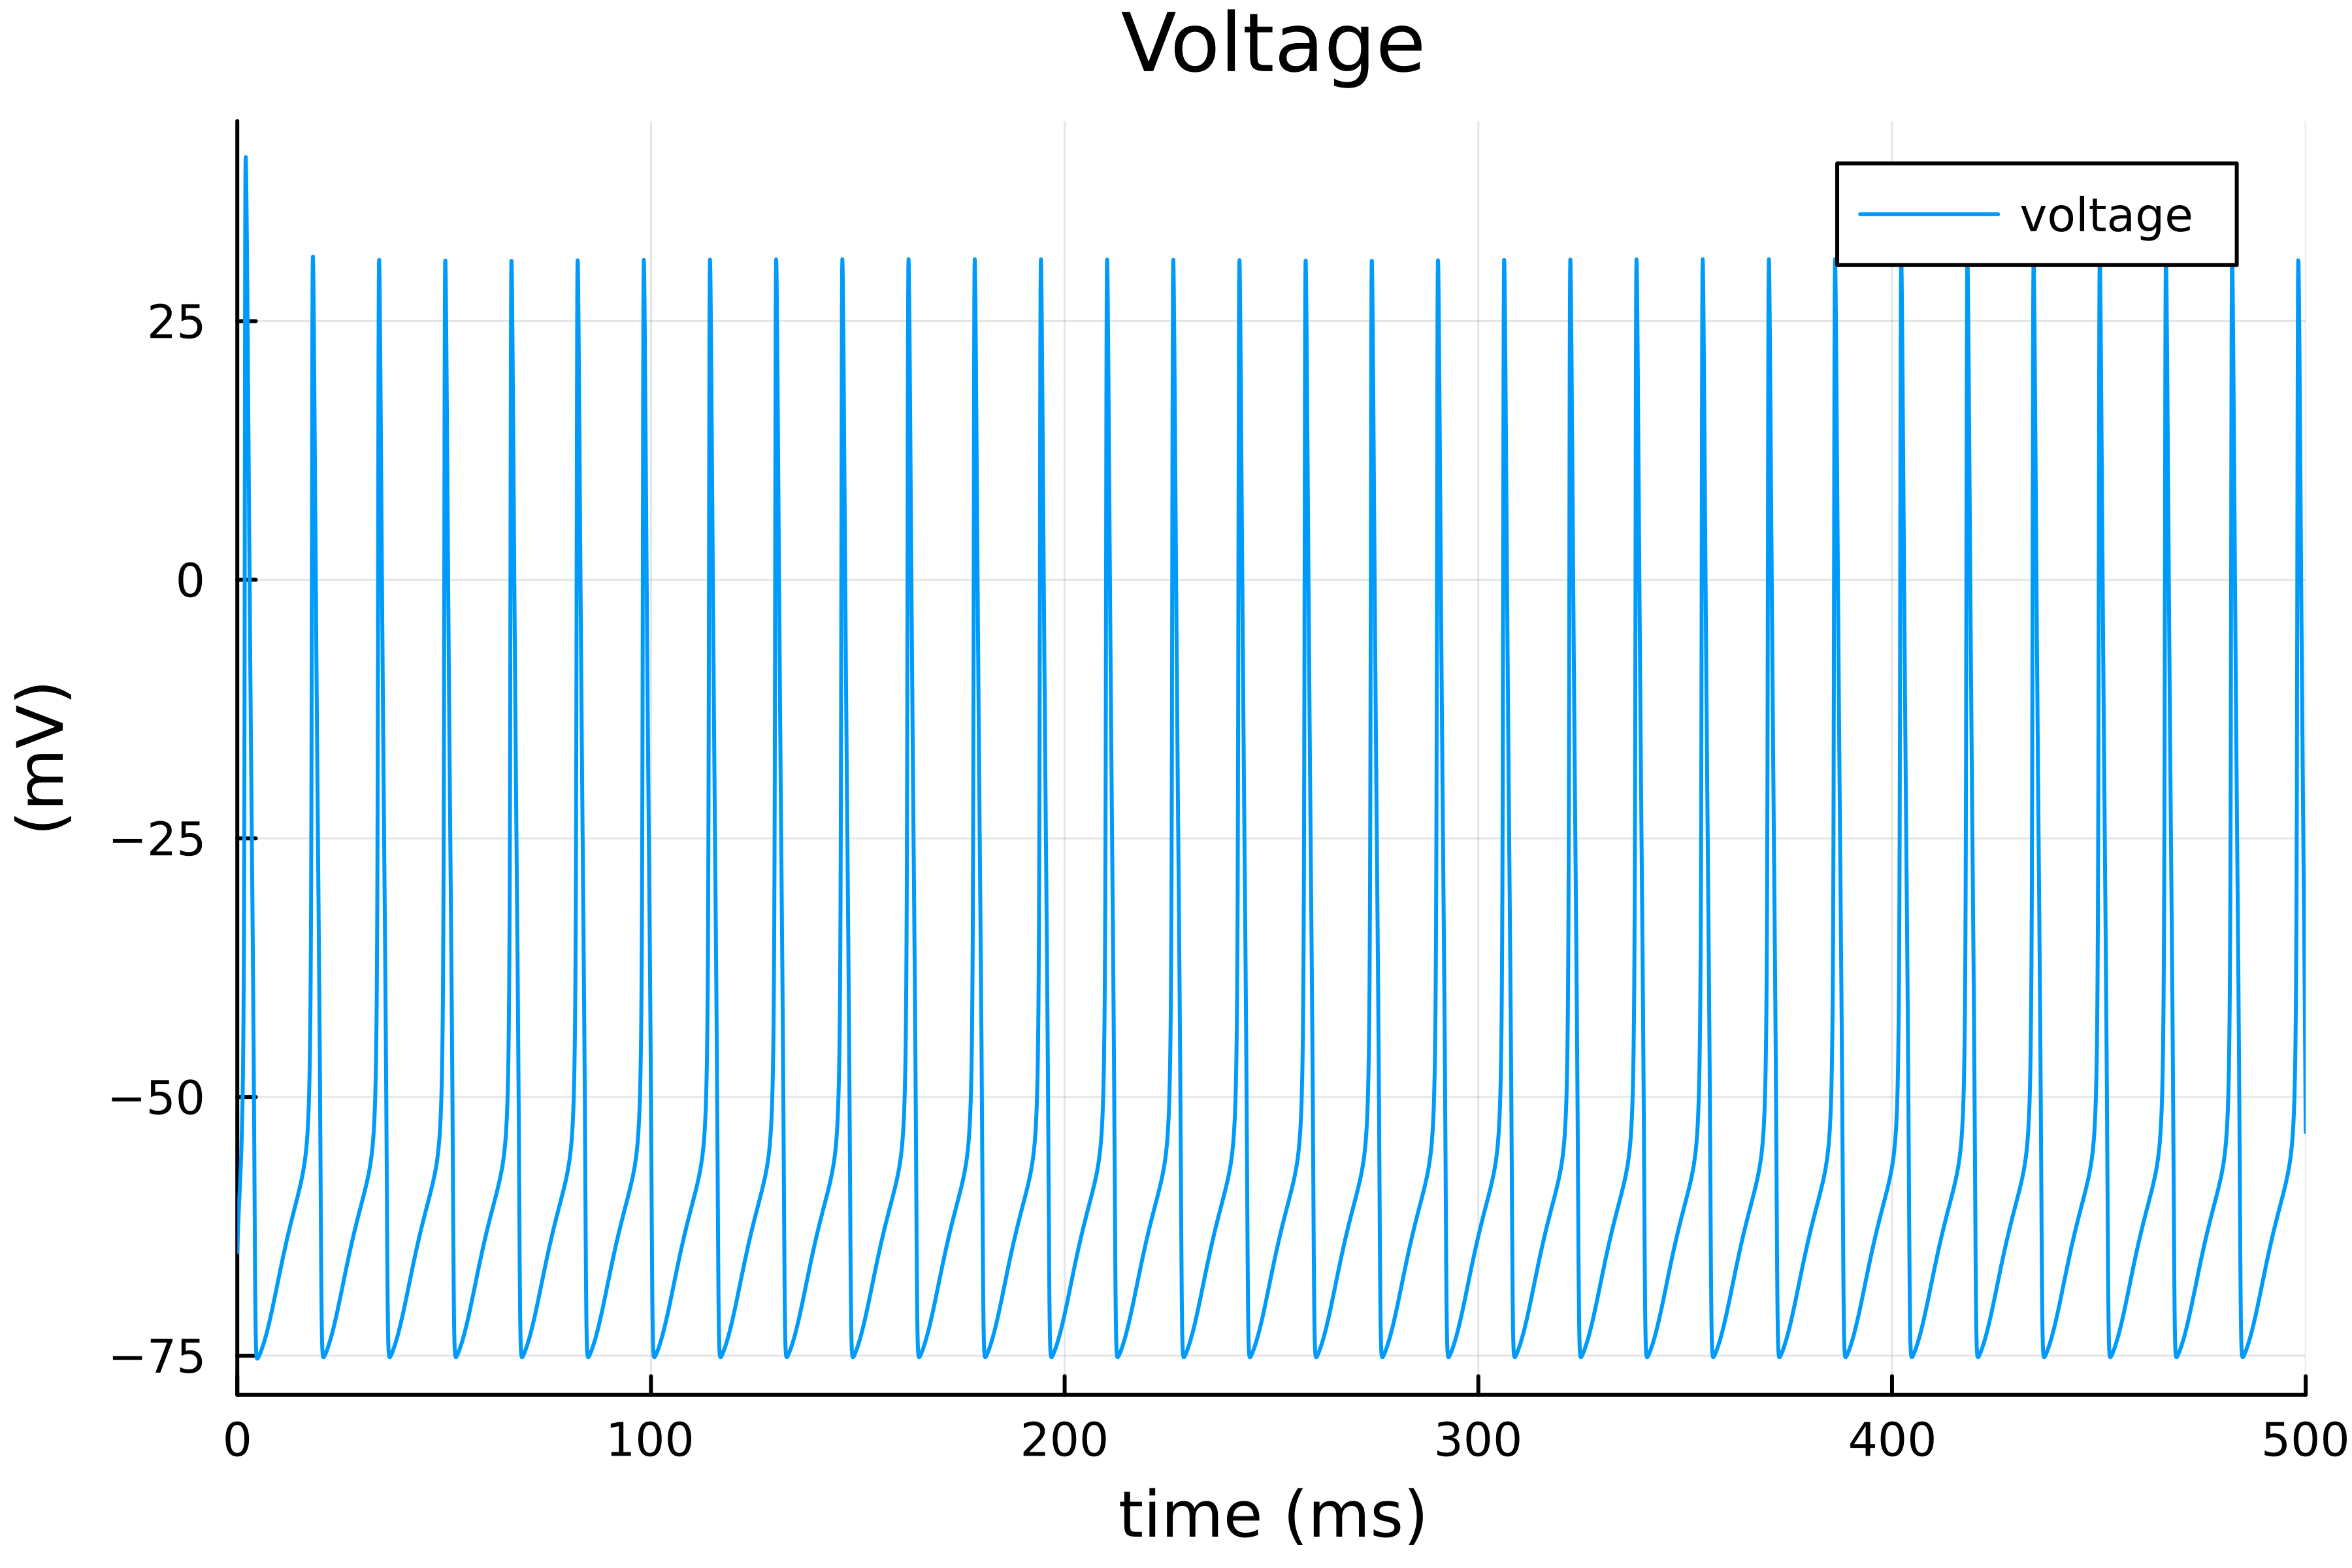
\includegraphics[width=0.75\columnwidth]{example.png}
    \caption{Caption.}
    \label{fig:LABEL}
\end{figure}

\end{document}
